\documentclass{beamer}

\usepackage[english]{babel}
\usepackage{amsmath,amsthm,amsfonts}
\usepackage{xkeyval}
\usepackage{graphics}
\usepackage{float}
\usepackage{url}
\usepackage{colortbl}%color a table
\usepackage[lined,boxed,linesnumbered]{algorithm2e}
\usepackage{CJKutf8}

\definecolor{mycolor}{RGB}{210,105,30}
\definecolor{mycolorlys}{RGB}{205,133,63}
\definecolor{mycolorlyslys}{RGB}{184,134,11}
\definecolor{mycolorlyslyslys}{RGB}{218,165,32}

\definecolor{rowcolor1}{RGB}{135,206,250}
\definecolor{rowcolor2}{RGB}{255,165,0}
\definecolor{rowcolor3}{RGB}{255,20,147}
\definecolor{rowcolor4}{RGB}{147,112,219}
\definecolor{rowcolor5}{RGB}{197,12,29}
\definecolor{rowcolor6}{RGB}{197,129,29}
%输入罗马数字
\newcommand{\myRoman}[1]{\uppercase\expandafter{\romannumeral#1}}
\newcommand{\myroman}[1]{\romannumeral#1}

\mode<presentation>
{
	\usetheme{Madrid}
	\usecolortheme[named=mycolor]{structure}
	\useinnertheme{rectangles}
	\useoutertheme{infolines}%default,infolines,miniframes,shadow,sidebar,smoothbars,smoothtree,split,tree
	\usefonttheme[onlymath]{serif}
	\setbeamercovered{transparent}
	\setbeamertemplate{blocks}[rounded][shadow=true]
	\setbeamertemplate{background}{
\includegraphics[height=\paperheight,width=\paperwidth]{images/BKG}}%设置背景图片
}

\title{Report on UFLDL-Part \myRoman{3}}
\author{Yunfei WANG}
\institute{\inst{1}School of Computer Science \& Technology \\ Huazhong University of Science \& Technology}
\date{June 25th, 2013}
%\logo{
\includegraphics[scale=0.07]{images/HUSTLogo}}

\begin{document}
\begin{CJK*}{UTF8}{gbsn}

\begin{frame}
\titlepage
\end{frame}

\begin{frame}\frametitle{Table of contents}
\tableofcontents
\end{frame}

\section{Overview}
\subsection{Advantages of Deep Networks}
\begin{frame}\frametitle{Advantages of Deep Networks}
\textcolor{blue}{Deep Networks have significantly greater representational power than a shallow one.}\\
\vspace{20pt}
\textcolor{red}{Learn part-whole decompositions}:
\begin{itemize}
\item \emph{First Layer}: Group together pixels to detect edges
\item \emph{Second Layer}: Group together edges to detect contours
\item \emph{Third Layer}: Group together contours to detect more objects.
\end{itemize}
\vspace{20pt}
\textcolor{magenta}{Note}: It's important to use on-linear activation function in hidden layers.(Because multiple layers of linear functions would compute only a linear function of the input)

\end{frame}

\subsection{Difficulty of Training Deep Architectures}
\begin{frame}\frametitle{Difficulty of Training Deep Architectures}
\begin{block}{Traditional strategy of training deep architectures}
\begin{itemize}
\item Randomly initialize weights of a deep network
\item Train the network on a labeled set with a supervised learning objective
\end{itemize}
\end{block}
\begin{enumerate}
\item Availability of data\\
The method above only relies on labeled data for training.\\
Difficult to obtain enough labeled examples to fit model parameters.\\
Training on insufficient data would result in overfitting.
\item Local Optima\\
Minimizing $\sum_i\|h_W(x^i)-y^i\|^2$ in a deep network turn out to be rife with bad local optima.Training with gradient descent,conjugate gradient or L-BFGS no longer work well.
\item Diffusion of Gradients\\
When using backpropagation to compute derivatives,gradients propagated backwards rapidly diminish in magnitude as the depth of network increases.Weights of earlier layers change slowly.
\end{enumerate}
\end{frame}

\subsection{Greedy Layer-wise Training}
\begin{frame}\frametitle{Greedy Layer-wise Training}
Main idea of greedy layer-wise training:
\begin{itemize}
\item Step 1:Train the layers of network one after another(supervised or unsupervised);
\item Step 2:Weights from training layers individually are used to initialize deep network
\item Step 3:Fine-tuning entire architecture
\end{itemize}
What does greedy layer-wise training bring to us?
\begin{itemize}
 \item Availability of data\\
 Massive unlabeled data is used to learn and discover patterns by self-taught learning.Compared with purely supervised approaches,this brings us much better classifiers.
 \item Better local optima\\
 Unlabeled data provides a significant amount of "prior" information about patterns of input data.Weights start at a better location in parameter space after pre-training than randomly initialization.
\end{itemize}
\end{frame}


\section{Stacked Autoencoders}
\begin{frame}[allowframebreaks]\frametitle{Stacked Autoencoders}
First, train a sparse autoencoder on raw inputs $x^k$ to learn primary features $h^{1,k}$
\begin{figure}
\centering
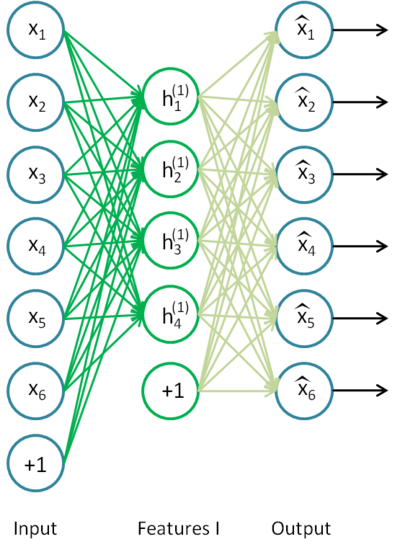
\includegraphics[scale=0.55]{images/Stacked_SparseAE_Features1}
\caption{1st-layer Autoencoder}
\end{figure}
Second, train a sparse autoencoder on primary features $h^{1,k}$ to learn second features $h^{2,k}$
\begin{figure}
\centering
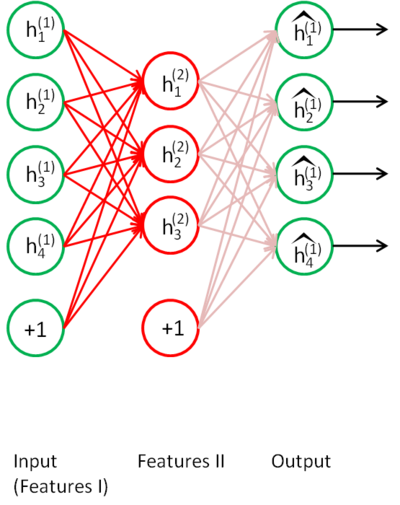
\includegraphics[scale=0.6]{images/Stacked_SparseAE_Features2}
\caption{2nd-layer Autoencoder}
\end{figure}
Next, train a softmax classifier on the last features $h^{2,k}$ to map them to digit labels.
\begin{figure}
\centering
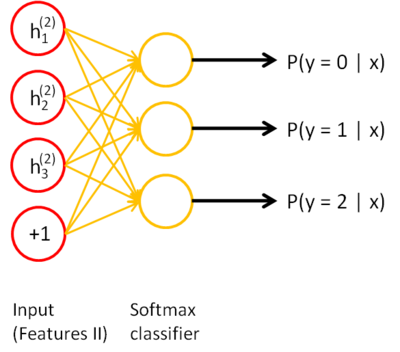
\includegraphics[scale=0.7]{images/Stacked_Softmax_Classifier}
\caption{Softmax Classifier in last layer}
\end{figure}
Finally, combine all layers to form a stacked autoencoder with 2 hidden layers and a final softmax classifier layer capable of classifying.
\begin{figure}
\centering
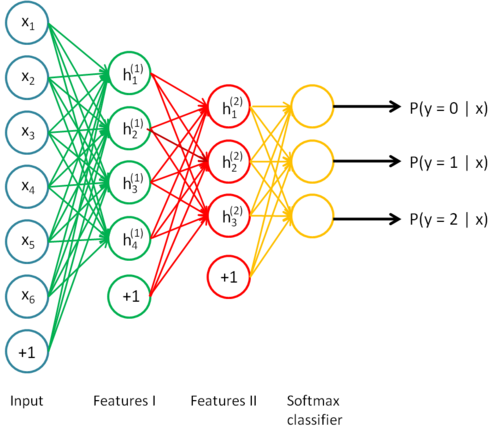
\includegraphics[scale=0.65]{images/Stacked_Combined}
\end{figure}
\end{frame}


\section{Fine-tuning Stacked AEs}
\begin{frame}\frametitle{Fine-tuning Stacked AEs}
Fine tuning treats all layers as a single model and tunes all weights in each iteration,greatly improving the performance of a stacked autoencoder.
\begin{algorithm}[H]
Perform a feedforward pass to compute activations for all layers\;
For output layer,set
\begin{equation}
\delta^L=-(\nabla_{a^L}J)\bullet f'(z^L)
\end{equation}
\For{$l=L-1,L-2,\cdots,2$}
{
\begin{equation}
\delta^l=((W^l)^T\delta^{l+1})\bullet f'(z^l)
\end{equation}
}
Computing partial derivations:
\begin{equation}
\nabla_{W^l}J(W,b;x,y)=\delta^{l+1}(a^l)^T
\end{equation}
\begin{equation}
\nabla_{b^l}J(W,b;x,y)=\delta^{l+1}
\end{equation}
\end{algorithm}
\end{frame}

\begin{frame}\frametitle{Experiments on Stacked AEs}
\begin{table}
\begin{tabular}{|c|c|c|}
\rowcolor{rowcolor1}
Dataset & Dimensionality & Number of Samples\\
\rowcolor{rowcolor2}
Training Data & $784$ & $60000$\\
\rowcolor{rowcolor3}
Testing Data & $784$ & $10000$\\
\end{tabular}
\caption{MNIST}
\end{table}
\begin{table}
\begin{tabular}{|c|c|c|}
\hline
\rowcolor{rowcolor1}
NUM of Autoencoders & Before Fine-tuning & After Fine-tuning\\
\hline
\rowcolor{rowcolor2}
$2$(Time=81min) & ACC=$87.83\%$ & ACC=$97.59\%$\\
\hline
\rowcolor{rowcolor3}
$3$(Time=106min) & ACC=$65.86\%$ & ACC=$97.35\%$\\
\hline
\rowcolor{rowcolor4}
$4$(Time=118min) & ACC=$11.35\%$ & ACC=$97.05\%$\\
\hline
\rowcolor{rowcolor5}
$5$(Time=83min) & ACC=$11.35\%$ & ACC=$11.35\%$\\
\hline
\rowcolor{rowcolor6}
$6$(Time=86min) & ACC=$11.35\%$ & ACC=$11.35\%$\\
\hline
\end{tabular}
\caption{Experiment Results}
\end{table}
\end{frame}

\end{CJK*}
\end{document}
